\medskip

Nomme le plus précisément possible chaque solide selon sa description ou sa représentation (en
perspective ou en développement) :
\medskip

\begin{tabularx}{\textwidth}{|X|X|}\hline
\textbf{Description ou représentation} & \textbf{Nom du solide} \\\hline
 \makecell[l]{Polyèdre à cinq faces :\\
  Trois rectangulaires et deux triangulaires.}
 & \\\hline
 Polyèdre à six faces rectangulaires.
 & \\\hline

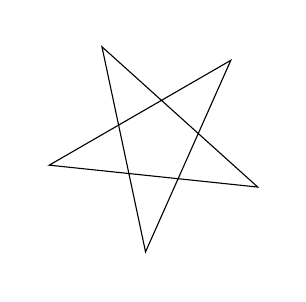
\begin{tikzpicture}[scale=0.7]
    \def\r{2}
    \def\n{5}
    \pgfmathsetmacro\m{\n-1}
    \foreach \i in {0,...,\n}
    \path ({90+\i*360/\n+30}:\r) coordinate (V\i);
    \draw (V2)--(V0)--(V3)--(V1)--(V4)--cycle;
    \foreach \i in {0,...,\m}{
    \path (0,0)--(V\i)--([turn]0:.4); 
    }
    \end{tikzpicture}
& \\\hline
    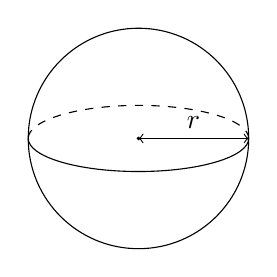
\begin{tikzpicture}[scale=0.7]
      %\shade[ball color = gray!40, opacity = 0.4] (0,0) circle (2cm);
      \draw (0,0) circle (2cm);
      \draw (-2,0) arc (180:360:2 and 0.6);
      \draw[dashed] (2,0) arc (0:180:2 and 0.6);
      \fill[fill=black] (0,0) circle (1pt);
      \draw[<->] (0,0 ) -- node[above]{$r$} (2,0);
    \end{tikzpicture}
& \\\hline

\end{tabularx}